\documentclass{beamer}
\setbeamercovered{transparent}
\usepackage{listings}
\usepackage[T1]{fontenc}
\usepackage{booktabs}

\usetheme[pageofpages=of,% String used between the current page and the
                         % total page count.
          bullet=circle,% Use circles instead of squares for bullets.
          titleline=true,% Show a line below the frame title.
          titlepagelogo=opensuse,
          alternativetitlepage=true,% Use the fancy title page.
          ]{Torino}


% Define some styles
\lstdefinestyle{mybash}{
  language=bash,
  basicstyle=\footnotesize\ttfamily,
  keywordstyle=\color{blue}\ttfamily,
  stringstyle=\color{red}\ttfamily,
  commentstyle=\color{green}\ttfamily,
  morecomment=[l][\color{magenta}]{\#}
}

\lstdefinestyle{myperl}{
  language=Perl,
  basicstyle=\footnotesize\ttfamily,
  keywordstyle=\color{blue}\ttfamily,
  stringstyle=\color{red}\ttfamily,
  commentstyle=\color{green}\ttfamily,
  morecomment=[l][\color{magenta}]{\#}
}

\lstdefinestyle{mypython}{
  language=Python,
  showstringspaces=false,
  basicstyle=\footnotesize\ttfamily,
  keywordstyle=\color{blue}\ttfamily,
  stringstyle=\color{red}\ttfamily,
  commentstyle=\color{green}\ttfamily,
  morecomment=[l][\color{magenta}]{\#}
}


% Counter commands for enumerates
\newcounter{saveenumi}
\newcommand{\seti}{\setcounter{saveenumi}{\value{enumi}}}
\newcommand{\conti}{\setcounter{enumi}{\value{saveenumi}}}


\setbeamerfont{title}{series=\bfseries,size=\LARGE}
\author{Alberto Planas <aplanas@suse.de>\newline {\small openSUSE Team}}
\title{How to Contribute to openQA -- oSC14}
\subtitle{A Fast Track to openQA Highway}


\AtBeginSection[]{
  \setbeamercolor{background canvas}{bg=chameleongreen3}
  \begin{frame}[plain]
    \begin{center}\begin{huge}\textcolor{white}{\secname}\end{huge}\end{center}
  \end{frame}
  \setbeamercolor{background canvas}{bg=}
}

\AtBeginSubsection[]{
  \setbeamercolor{background canvas}{bg=chameleongreen3}
  \begin{frame}[plain]
    \begin{center}\begin{huge}\textcolor{white}{\subsecname}\end{huge}\end{center}
  \end{frame}
  \setbeamercolor{background canvas}{bg=}
}


\begin{document}

\begin{frame}[t,plain]
  \titlepage
\end{frame}


\section{Introduction}

\begin{frame}{TL;DR}
  If you want to contribute to openQA:
  \begin{itemize}
  \item Take the code
  \item Learn Perl, Mojolicious or any of the other libraries
  \item Go to the project {\em progress} page
  \item Take an Easy Task or any other task
  \item Hack, hack, ...
  \item Create a pull request to into Github
  \end{itemize}
\end{frame}

\begin{frame}{What is openQA}
  With openQA we can test the installation process of a distribution.
  \begin{itemize}
  \item We provide the tests (Perl code)
  \item We provide the ISO image
  \item A worker will launch an instance of os-autoinst
  \item os-autoinst create the environment
    \begin{itemize}
    \item Environment variables
    \item HDD images
    \end{itemize}
  \item ... and run the tests
  \end{itemize}
\end{frame}

\begin{frame}{Architecture}
  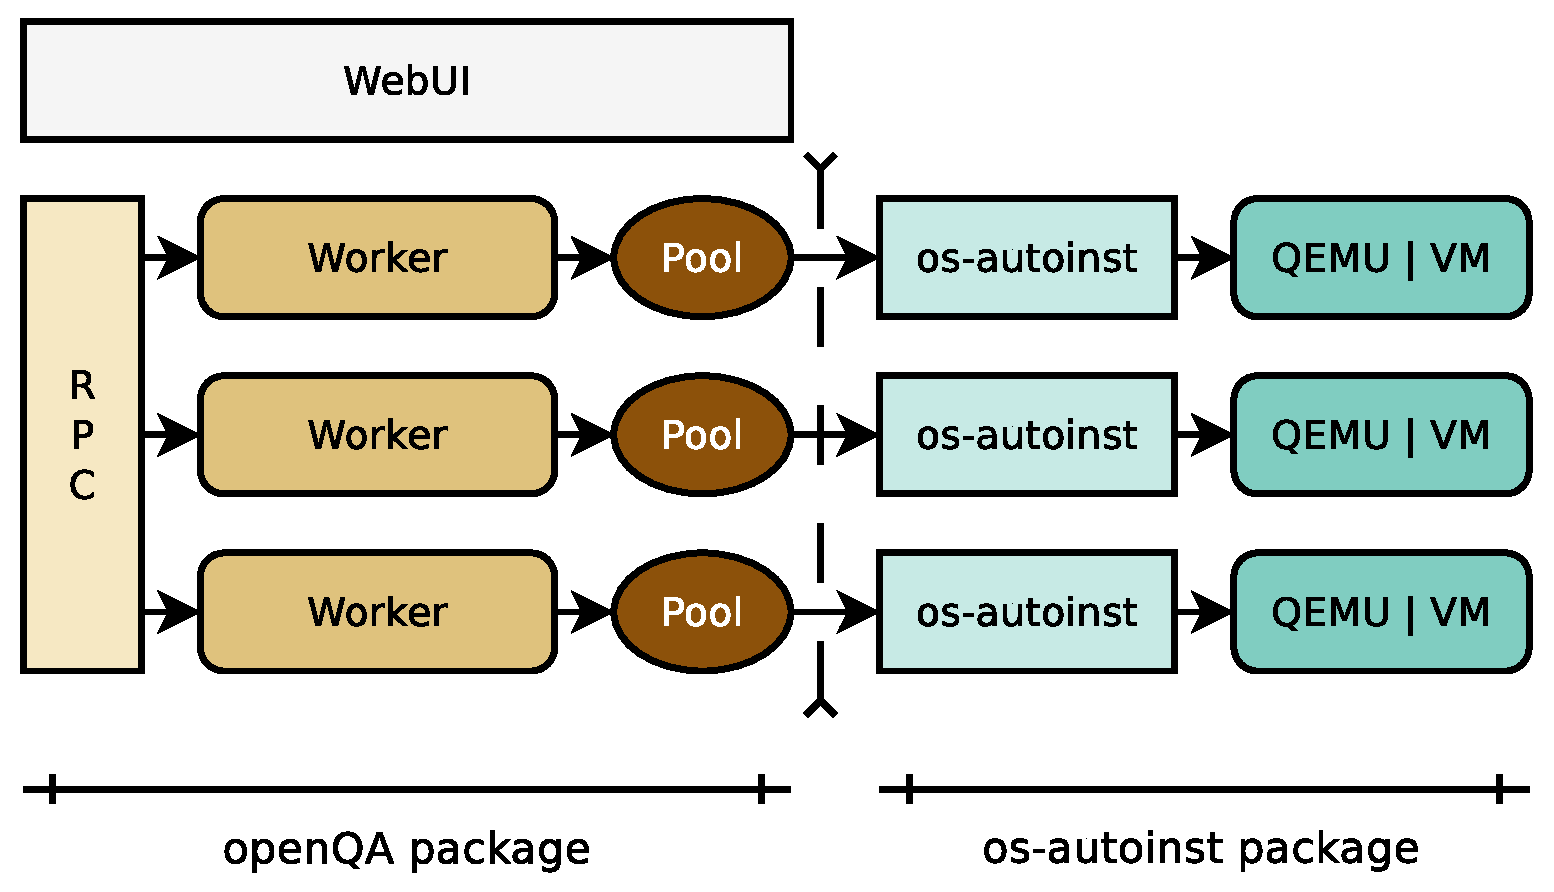
\includegraphics[height=5.8cm,width=10.3cm]{arch}
\end{frame}


\section{Technologies}

\begin{frame}{Main Technologies}
  \begin{itemize}
  \item openQA and os-autoinst are written in Perl
  \item Learn Perl in about 2 hours 30 minutes\newline
    {\small\url{http://qntm.org/files/perl/perl.html}}
    \item The user interface (openQA) use to big libraries
      \begin{itemize}
      \item Mojolicious. A Sinatra-like web framework for Perl\newline
        {\small\url{http://mojolicio.us/}}
      \item DBIx::Class. ORB and Schema abstraction layer for Perl\newline
        {\small\url{http://www.dbix-class.org/}}
      \end{itemize}
  \item QEMU to create VM and configure machines
  \end{itemize}
\end{frame}

\begin{frame}{Getting openQA}
  \begin{itemize}
  \item Everything is in github:
    \begin{itemize}
    \item openQA UI:\newline
      {\small\url{https://github.com/os-autoinst/openQA}}
    \item os-autoinst:\newline
      {\small\url{https://github.com/os-autoinst/os-autoinst}}
    \item Installation instructions:\newline
      {\small\url{https://github.com/os-autoinst/openQA/blob/master/docs/Installation.asciidoc}}
    \end{itemize}
  \item Compare your installation with\newline
    {\small\url{https://openqa.opensuse.org/}}
  \end{itemize}
\end{frame}


\section{Easy Tasks}

\begin{frame}{Control Tool}
  \begin{itemize}
  \item We are using a tool to control the project development\newline
    {\small\url{https://progress.opensuse.org/projects/openqav3}}
  \item Use this tool to communicate with the team, and inform of your progress
  \item And we prepare a list of tasks that can be done by you\newline
    {\small\url{https://progress.opensuse.org/versions/73}}
  \end{itemize}
\end{frame}

\begin{frame}{Some Easy Hacks}
  \begin{itemize}
  \item action \#2208: pagination in job listing\newline
    Very good tasks to learn about Mojolicious. Many of the list views
    needs a pagination mechanism.\newline
    {\small\url{https://progress.opensuse.org/issues/2208}}
  \item action \#2248: Complete bootstrap/install process\newline
    Ideal to dig into the deployment. We want an easy way to bootstrap
    and deploy the application.\newline
    {\small\url{https://progress.opensuse.org/issues/2248}}
  \item action \#2238: better details for scheduled jobs\newline
    If you want to improve the UX, this is your task.\newline
    {\small\url{https://progress.opensuse.org/issues/2238}}
  \end{itemize}
\end{frame}


\section{End Note}

\begin{frame}{SUSE is hiring}
  \begin{figure}
    \includegraphics[width=0.8\linewidth]{suse_hiring.png}
  \end{figure}
\end{frame}

\begin{frame}{Thanks}
  \begin{center}
    Thank you for your attention.
  \end{center}
\end{frame}

\end{document}
